\documentclass[11pt]{beamer}
\useoutertheme{infolines}
\setbeamertemplate{headline}

\useinnertheme{default}
\usecolortheme{orchid}


\usepackage[utf8]{inputenc}
\usepackage[english]{babel}
\usepackage{amsmath}
\usepackage{amsfonts}
\usepackage{amssymb}
\usepackage{graphicx}
\graphicspath{{../imgs/}}
\usepackage{hyperref}
\urlstyle{same}

% units
\usepackage{siunitx}
\sisetup{
  locale = DE ,
  per-mode = symbol
}
% tikz pakete für die Erstellung von plots:
\usepackage{tikz}
\usetikzlibrary{positioning}
\usetikzlibrary{fpu}
% \usetikzlibrary{intersections}
% \usetikzlibrary{math}
\usepackage{pgfplots}
\usepgfplotslibrary{groupplots}
\usepgfplotslibrary{units}
\usepackage{tikz-timing} % für timing-diagramme:
\pgfplotsset{compat=newest, unit code/.code 2 args={\si{#1#2}}}

% für hyperlinks:
\usepackage{hyperref}

%\usepackage{xcolor}

\usepackage{xintbinhex}

\usepackage[
backend=bibtex,
sortcites=false,
style=numeric,
firstinits=true,
uniquename=init,
isbn=false,
pagetracker=false,
maxbibnames=50,
maxcitenames=3,
autocite=inline,
block=space,
backref=false,
backrefstyle=three+,
date=short,
url=false,
doi=true,
eprint=false,
sorting=none
]{biblatex}
\addbibresource{refs.bib}

\usefonttheme[onlymath]{serif}

% hexcounter
\newcounter{hexcount}
\newcommand{\hexcountmakro}{
  \xintDecToHex{\the\value{hexcount}}
  \ifnum \value{hexcount}=15
    \setcounter{hexcount}{0}
  \else
    \addtocounter{hexcount}{1}
  \fi
}

\author{Markus Hartlage}
\title[Digitaler Funktionsgenerator in VHDL]{Entwicklung und Implementierung eines digitalen Funktionsgenerators in VHDL}
%\setbeamercovered{transparent} 
%\setbeamertemplate{navigation symbols}{} 
\titlegraphic{
\includegraphics[width=3cm]{logo.png}}
\institute{FH-Bielefeld} 
%\date{} 
%\subject{}
\begin{document}

\begin{frame}
  \titlepage
\end{frame}

% Konzept
% Konfiguration - hier kann ich vielleicht das python Interface zeigen
% Funktionskomponenten
% Funktionstests
% Fazit

% \begin{frame}
%   \tableofcontents
% \end{frame}

\section{Konzept}

\begin{frame}{Konzept - Anforderungen}
  \begin{itemize}
    \item Ausgabe vier verschiedener Funktionsverläufe
      \begin{itemize}
        \item Konstante, Rechteck, Zick-Zack, Rampe
      \end{itemize}
    \item Konfiguration per UART-Schnittstelle
      \begin{itemize}
        \item high- und low-Wert, Zykluszeit, dutycycle, Flankensteigung
      \end{itemize}
  \end{itemize}

  \begin{figure}
    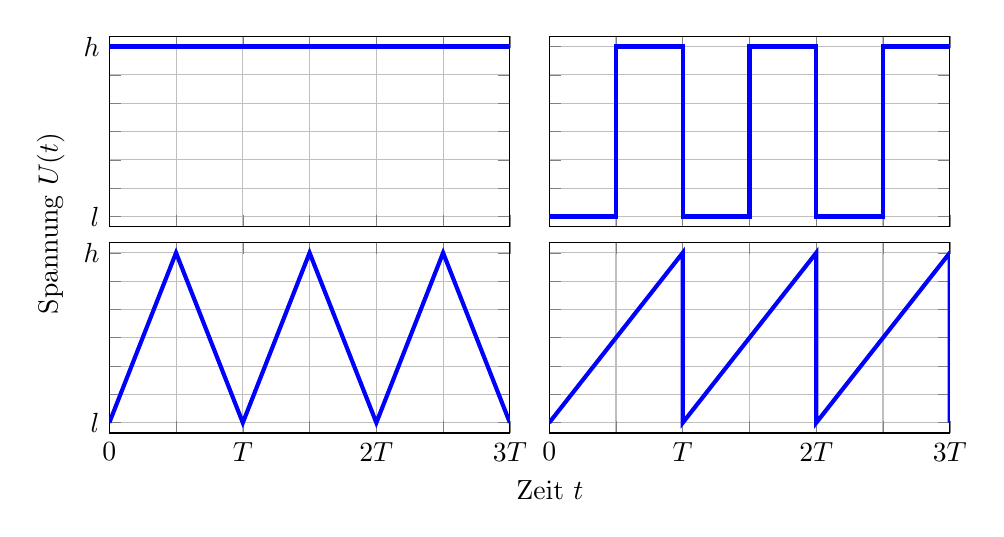
\begin{tikzpicture}
      \pgfplotsset{
        xtick={0, 15, 30, 45, 60, 75, 90},
        ytick={0, 0.55, 1.1, 1.65, 2.2, 2.75, 3.3},
        xmin=0, xmax=90,
        ymin=-0.2, ymax=3.5,
        xticklabels={$0$, , $T$, , $2T$, , $3T$,},
        yticklabels={$l$, , , , , ,$h$}, 
        grid=major,
        width=0.55\textwidth,
        height=0.33\textwidth}
      \begin{groupplot}[group style={
          group size=2 by 2,
          x descriptions at=edge bottom,
          xlabels at=edge bottom,
          y descriptions at=edge left,
          horizontal sep=0.5cm,
          vertical sep=0.2cm}]
        \nextgroupplot
        \addplot[color=blue, line width=1.5pt] coordinates{(0, 3.3)(90, 3.3)};
        \nextgroupplot
        \addplot[color=blue, line width=1.5pt] coordinates{(0, 0)(15, 0)(15, 3.3)(30, 3.3)(30, 0)(45, 0)(45, 3.3)(60, 3.3)(60, 0)(75, 0)(75, 3.3)(90, 3.3)};
        \nextgroupplot[
        xlabel=Zeit $t$,
        every axis x label/.append style={at=(ticklabel cs:1.1)},
        ylabel=Spannung $U(t)$,
        every axis y label/.append style={at=(ticklabel cs:1.1)}] 
        \addplot[color=blue, line width=1.5pt] coordinates{(0, 0)(15, 3.3)(30, 0)(45, 3.3)(60, 0)(75, 3.3)(90, 0)};
        \nextgroupplot
        \addplot[color=blue, domain=0:90, line width=1.5pt]  coordinates{(0, 0)(30, 3.3)(30, 0)(60, 3.3)(60, 0)(90, 3.3)(90, 0)};
      \end{groupplot}
    \end{tikzpicture}
  \end{figure}
\end{frame}

\begin{frame}{Konzept - Aufbau}
  \begin{itemize}
    \item Aufbau aus Konfigurations-, Funktions- und DAC Komponente
    \item zusätzliche Hardware: Uart-Interface und digital-analog Konverter
  \end{itemize}

  \begin{figure}
    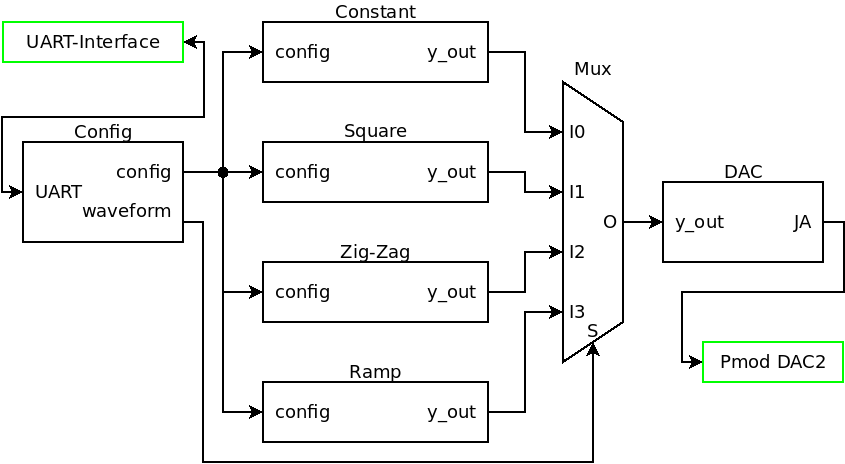
\includegraphics[scale=0.36]{fg_diagram_pres}
  \end{figure}
\end{frame}

\section{Komponenten}

\begin{frame}[t]{Komponenten - Rampe}
  \begin{figure}
    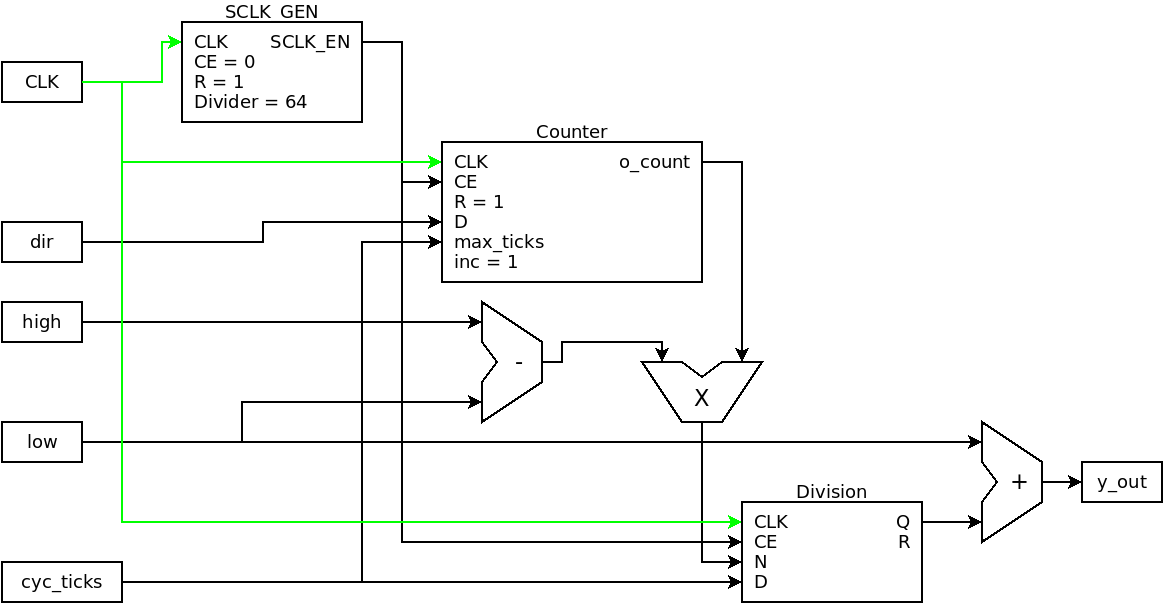
\includegraphics[scale=0.28]{ramp}
  \end{figure}
  \begin{itemize}
    \item Abbildung des 24 Bit Zählstands auf 12 Bit Ausgang:
    $$ y\_out = (high - low) \cdot o\_count \div cyc\_ticks $$
  \end{itemize}
\end{frame}

\begin{frame}[t]{Komponenten - Rampe}
  \begin{figure}
    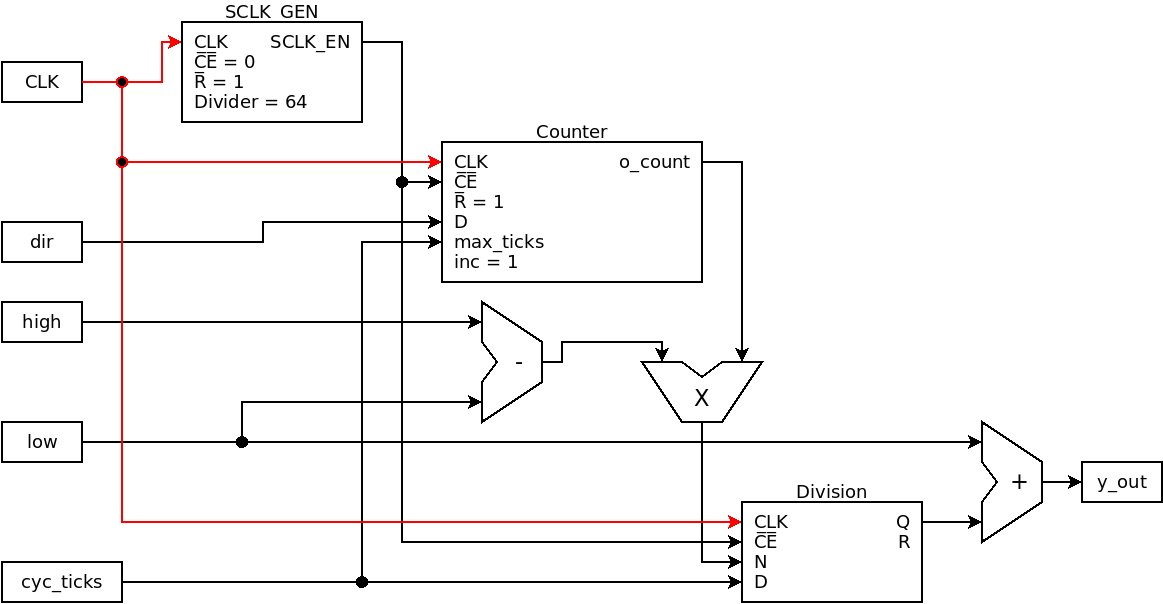
\includegraphics[scale=0.28]{ramp_step0}
  \end{figure}
  \begin{itemize}
    \item  Abzählen von 68 Taktzyklen
  \end{itemize}
\end{frame}

\begin{frame}[t]{Komponenten - Rampe}
  \begin{figure}
    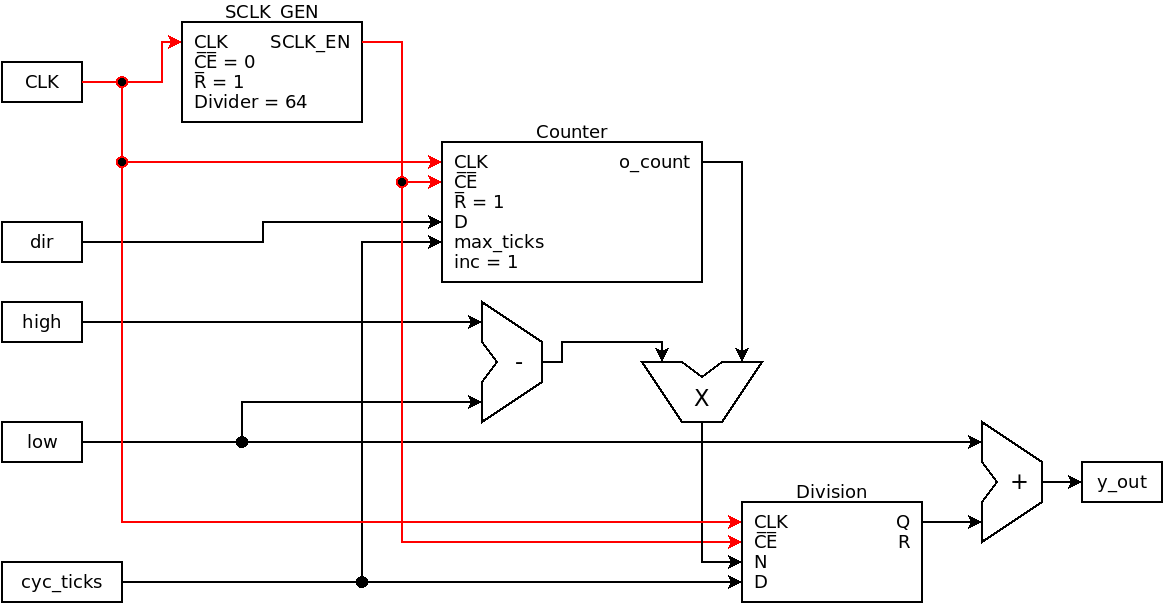
\includegraphics[scale=0.28]{ramp_step1}
  \end{figure}
  \begin{itemize}
    \item Aktivieren von \emph{Counter} und \emph{Division}
  \end{itemize}
\end{frame}

\begin{frame}[t]{Komponenten - Rampe}
  \begin{figure}
    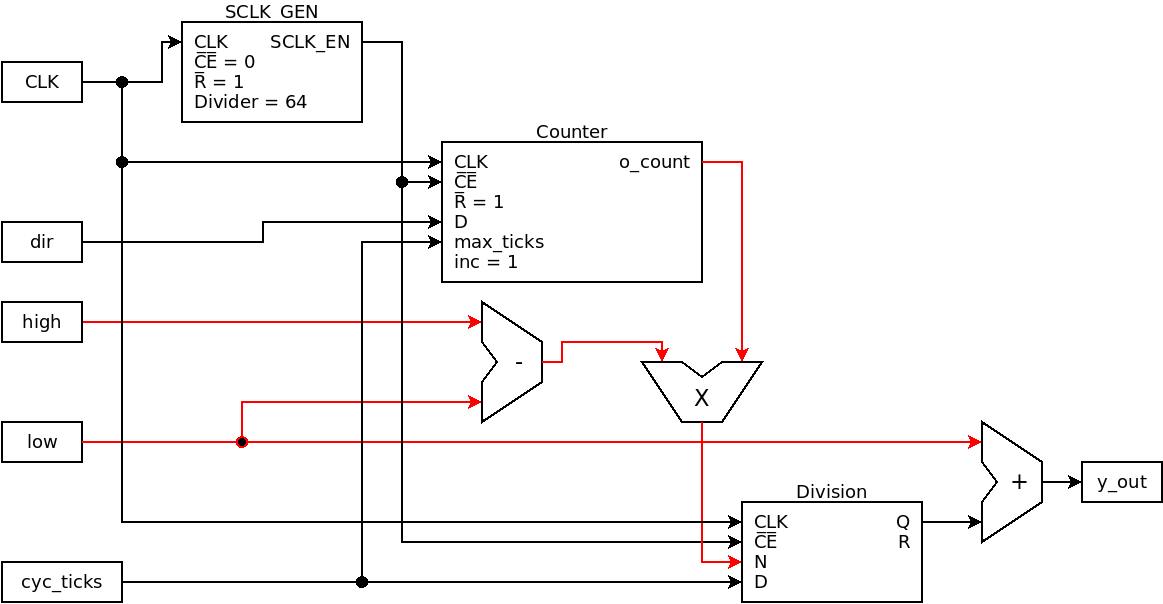
\includegraphics[scale=0.28]{ramp_step2}
  \end{figure}
  \begin{itemize}
    \item neuer Zählstand wird mit Amplitude multipliziert und \emph{Division} beginnt zu teilen
  \end{itemize}
\end{frame}

\begin{frame}[t]{Komponenten - Rampe}
  \begin{figure}
    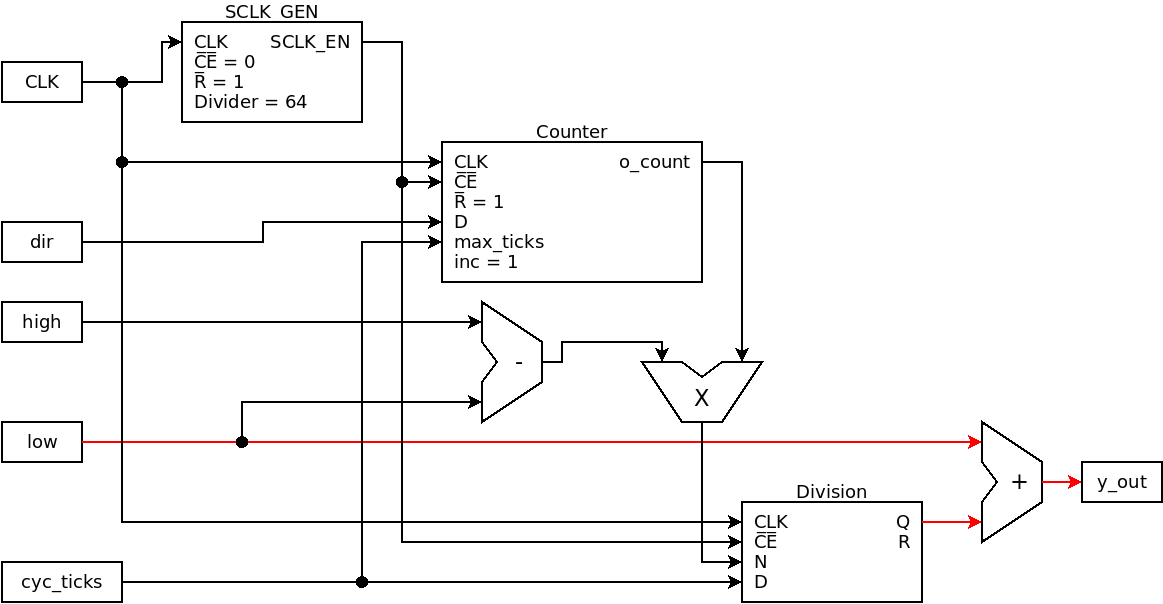
\includegraphics[scale=0.28]{ramp_step3}
  \end{figure}
  \begin{itemize}
    \item untere zwölf Bits von \emph{Q} plus \emph{low} ergeben \emph{y\_out}
  \end{itemize}
\end{frame}

\begin{frame}{Komponenten - Zick-Zack}
  \begin{itemize}
    \item Zählrichtung wird mit Komperatoren geregelt
    \item halbe Zykluszeit (\emph{cyc\_ticks} um ein Bit nach rechts geschoben)
  \end{itemize}
  \begin{figure}
    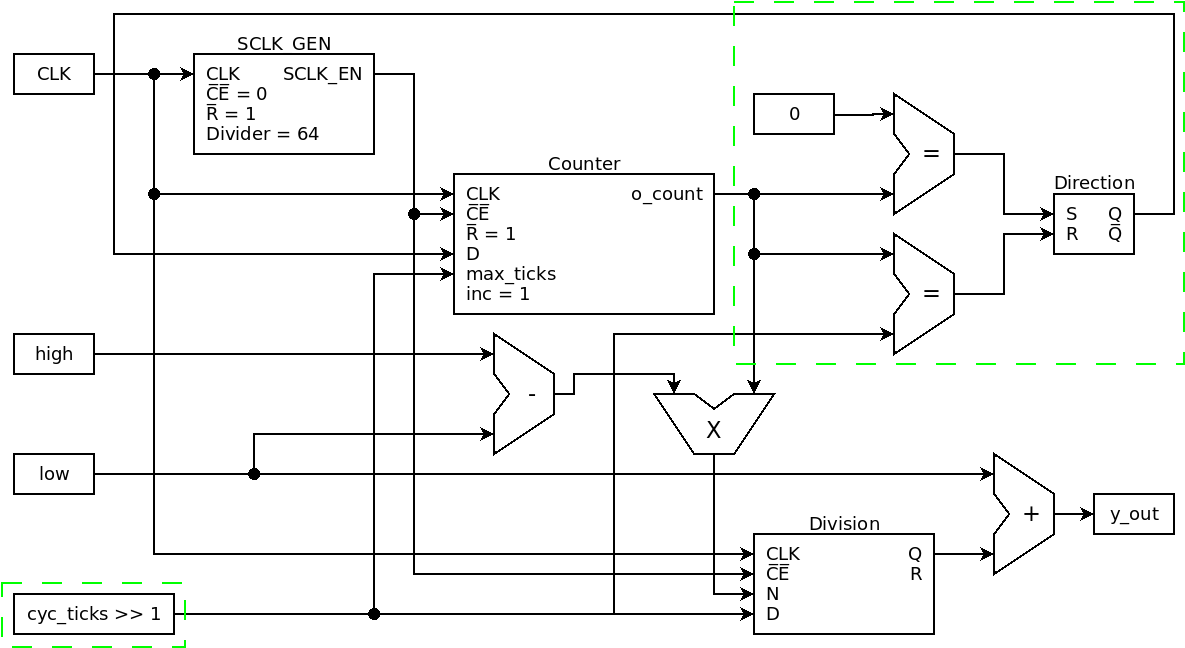
\includegraphics[scale=0.28]{zigzag}
  \end{figure}
\end{frame}

\begin{frame}{Komponenten - Konfiguration}
  Aufbau als state machine:
  \begin{itemize}
  \item Byteweises Einlesen der UART Rx Signale 
  \item Interpretation von vier Bytes als Befehl (Befehlscode + Argumente) 
  \item Berechnung und Speicherung der neuen Konfiguration
  \end{itemize}
  \resizebox{\textwidth}{!}{
    % Graphic for TeX using PGF
% Title: /home/markus/Documents/FH/function_generator_doku/imgs/config_state_machine.dia
% Creator: Dia v0.97+git
% CreationDate: Fri Apr  1 14:09:59 2022
% For: markus
% \usepackage{tikz}
% The following commands are not supported in PSTricks at present
% We define them conditionally, so when they are implemented,
% this pgf file will use them.
\ifx\du\undefined
  \newlength{\du}
\fi
\setlength{\du}{15\unitlength}
\begin{tikzpicture}[even odd rule]
\pgftransformxscale{1.000000}
\pgftransformyscale{-1.000000}
\definecolor{dialinecolor}{rgb}{0.000000, 0.000000, 0.000000}
\pgfsetstrokecolor{dialinecolor}
\pgfsetstrokeopacity{1.000000}
\definecolor{diafillcolor}{rgb}{1.000000, 1.000000, 1.000000}
\pgfsetfillcolor{diafillcolor}
\pgfsetfillopacity{1.000000}
\pgfsetlinewidth{0.100000\du}
\pgfsetdash{}{0pt}
{\pgfsetcornersarced{\pgfpoint{1.000000\du}{1.000000\du}}\definecolor{diafillcolor}{rgb}{1.000000, 1.000000, 1.000000}
\pgfsetfillcolor{diafillcolor}
\pgfsetfillopacity{1.000000}
\fill (20.869812\du,5.684261\du)--(20.869812\du,7.813150\du)--(24.869812\du,7.813150\du)--(24.869812\du,5.684261\du)--cycle;
}{\pgfsetcornersarced{\pgfpoint{1.000000\du}{1.000000\du}}\definecolor{dialinecolor}{rgb}{0.000000, 0.000000, 0.000000}
\pgfsetstrokecolor{dialinecolor}
\pgfsetstrokeopacity{1.000000}
\draw (20.869812\du,5.684261\du)--(20.869812\du,7.813150\du)--(24.869812\du,7.813150\du)--(24.869812\du,5.684261\du)--cycle;
}% setfont left to latex
\definecolor{dialinecolor}{rgb}{0.000000, 0.000000, 0.000000}
\pgfsetstrokecolor{dialinecolor}
\pgfsetstrokeopacity{1.000000}
\definecolor{diafillcolor}{rgb}{0.000000, 0.000000, 0.000000}
\pgfsetfillcolor{diafillcolor}
\pgfsetfillopacity{1.000000}
\node[anchor=base,inner sep=0pt, outer sep=0pt,color=dialinecolor] at (22.869812\du,7.022532\du){IDLE};
\pgfsetlinewidth{0.100000\du}
\pgfsetdash{}{0pt}
{\pgfsetcornersarced{\pgfpoint{1.000000\du}{1.000000\du}}\definecolor{diafillcolor}{rgb}{1.000000, 1.000000, 1.000000}
\pgfsetfillcolor{diafillcolor}
\pgfsetfillopacity{1.000000}
\fill (8.869893\du,12.560686\du)--(8.869893\du,14.689574\du)--(13.551683\du,14.689574\du)--(13.551683\du,12.560686\du)--cycle;
}{\pgfsetcornersarced{\pgfpoint{1.000000\du}{1.000000\du}}\definecolor{dialinecolor}{rgb}{0.000000, 0.000000, 0.000000}
\pgfsetstrokecolor{dialinecolor}
\pgfsetstrokeopacity{1.000000}
\draw (8.869893\du,12.560686\du)--(8.869893\du,14.689574\du)--(13.551683\du,14.689574\du)--(13.551683\du,12.560686\du)--cycle;
}% setfont left to latex
\definecolor{dialinecolor}{rgb}{0.000000, 0.000000, 0.000000}
\pgfsetstrokecolor{dialinecolor}
\pgfsetstrokeopacity{1.000000}
\definecolor{diafillcolor}{rgb}{0.000000, 0.000000, 0.000000}
\pgfsetfillcolor{diafillcolor}
\pgfsetfillopacity{1.000000}
\node[anchor=base,inner sep=0pt, outer sep=0pt,color=dialinecolor] at (11.210788\du,13.898957\du){OUTPUT};
\pgfsetlinewidth{0.100000\du}
\pgfsetdash{}{0pt}
{\pgfsetcornersarced{\pgfpoint{1.000000\du}{1.000000\du}}\definecolor{diafillcolor}{rgb}{1.000000, 1.000000, 1.000000}
\pgfsetfillcolor{diafillcolor}
\pgfsetfillopacity{1.000000}
\fill (44.158474\du,13.173233\du)--(44.158474\du,15.302121\du)--(50.715974\du,15.302121\du)--(50.715974\du,13.173233\du)--cycle;
}{\pgfsetcornersarced{\pgfpoint{1.000000\du}{1.000000\du}}\definecolor{dialinecolor}{rgb}{0.000000, 0.000000, 0.000000}
\pgfsetstrokecolor{dialinecolor}
\pgfsetstrokeopacity{1.000000}
\draw (44.158474\du,13.173233\du)--(44.158474\du,15.302121\du)--(50.715974\du,15.302121\du)--(50.715974\du,13.173233\du)--cycle;
}% setfont left to latex
\definecolor{dialinecolor}{rgb}{0.000000, 0.000000, 0.000000}
\pgfsetstrokecolor{dialinecolor}
\pgfsetstrokeopacity{1.000000}
\definecolor{diafillcolor}{rgb}{0.000000, 0.000000, 0.000000}
\pgfsetfillcolor{diafillcolor}
\pgfsetfillopacity{1.000000}
\node[anchor=base,inner sep=0pt, outer sep=0pt,color=dialinecolor] at (47.437224\du,14.511504\du){INTERPRETE};
\pgfsetlinewidth{0.100000\du}
\pgfsetdash{}{0pt}
{\pgfsetcornersarced{\pgfpoint{1.000000\du}{1.000000\du}}\definecolor{diafillcolor}{rgb}{1.000000, 1.000000, 1.000000}
\pgfsetfillcolor{diafillcolor}
\pgfsetfillopacity{1.000000}
\fill (38.346874\du,5.630771\du)--(38.346874\du,7.759660\du)--(42.346874\du,7.759660\du)--(42.346874\du,5.630771\du)--cycle;
}{\pgfsetcornersarced{\pgfpoint{1.000000\du}{1.000000\du}}\definecolor{dialinecolor}{rgb}{0.000000, 0.000000, 0.000000}
\pgfsetstrokecolor{dialinecolor}
\pgfsetstrokeopacity{1.000000}
\draw (38.346874\du,5.630771\du)--(38.346874\du,7.759660\du)--(42.346874\du,7.759660\du)--(42.346874\du,5.630771\du)--cycle;
}% setfont left to latex
\definecolor{dialinecolor}{rgb}{0.000000, 0.000000, 0.000000}
\pgfsetstrokecolor{dialinecolor}
\pgfsetstrokeopacity{1.000000}
\definecolor{diafillcolor}{rgb}{0.000000, 0.000000, 0.000000}
\pgfsetfillcolor{diafillcolor}
\pgfsetfillopacity{1.000000}
\node[anchor=base,inner sep=0pt, outer sep=0pt,color=dialinecolor] at (40.346874\du,6.969043\du){SHIFT};
\pgfsetlinewidth{0.100000\du}
\pgfsetdash{}{0pt}
{\pgfsetcornersarced{\pgfpoint{1.000000\du}{1.000000\du}}\definecolor{diafillcolor}{rgb}{1.000000, 1.000000, 1.000000}
\pgfsetfillcolor{diafillcolor}
\pgfsetfillopacity{1.000000}
\fill (23.926163\du,16.086808\du)--(23.926163\du,18.215697\du)--(30.161163\du,18.215697\du)--(30.161163\du,16.086808\du)--cycle;
}{\pgfsetcornersarced{\pgfpoint{1.000000\du}{1.000000\du}}\definecolor{dialinecolor}{rgb}{0.000000, 0.000000, 0.000000}
\pgfsetstrokecolor{dialinecolor}
\pgfsetstrokeopacity{1.000000}
\draw (23.926163\du,16.086808\du)--(23.926163\du,18.215697\du)--(30.161163\du,18.215697\du)--(30.161163\du,16.086808\du)--cycle;
}% setfont left to latex
\definecolor{dialinecolor}{rgb}{0.000000, 0.000000, 0.000000}
\pgfsetstrokecolor{dialinecolor}
\pgfsetstrokeopacity{1.000000}
\definecolor{diafillcolor}{rgb}{0.000000, 0.000000, 0.000000}
\pgfsetfillcolor{diafillcolor}
\pgfsetfillopacity{1.000000}
\node[anchor=base,inner sep=0pt, outer sep=0pt,color=dialinecolor] at (27.043663\du,17.425079\du){CALCULATE};
\pgfsetlinewidth{0.100000\du}
\pgfsetdash{}{0pt}
\definecolor{diafillcolor}{rgb}{0.000000, 0.000000, 0.000000}
\pgfsetfillcolor{diafillcolor}
\pgfsetfillopacity{1.000000}
\pgfpathellipse{\pgfpoint{15.725894\du}{6.854147\du}}{\pgfpoint{0.500000\du}{0\du}}{\pgfpoint{0\du}{0.500000\du}}
\pgfusepath{fill}
\pgfsetlinewidth{0.100000\du}
\pgfsetdash{}{0pt}
\pgfsetbuttcap
{
\definecolor{diafillcolor}{rgb}{0.000000, 0.000000, 0.000000}
\pgfsetfillcolor{diafillcolor}
\pgfsetfillopacity{1.000000}
% was here!!!
\pgfsetarrowsend{stealth}
\definecolor{dialinecolor}{rgb}{0.000000, 0.000000, 0.000000}
\pgfsetstrokecolor{dialinecolor}
\pgfsetstrokeopacity{1.000000}
\draw (24.869812\du,5.684261\du)--(38.346874\du,5.630771\du);
}
% setfont left to latex
\definecolor{dialinecolor}{rgb}{0.000000, 0.000000, 0.000000}
\pgfsetstrokecolor{dialinecolor}
\pgfsetstrokeopacity{1.000000}
\definecolor{diafillcolor}{rgb}{0.000000, 0.000000, 0.000000}
\pgfsetfillcolor{diafillcolor}
\pgfsetfillopacity{1.000000}
\node[anchor=base,inner sep=0pt, outer sep=0pt,color=dialinecolor] at (31.608343\du,5.444530\du){UART\_rdy=0};
% setfont left to latex
\definecolor{dialinecolor}{rgb}{0.000000, 0.000000, 0.000000}
\pgfsetstrokecolor{dialinecolor}
\pgfsetstrokeopacity{1.000000}
\definecolor{diafillcolor}{rgb}{0.000000, 0.000000, 0.000000}
\pgfsetfillcolor{diafillcolor}
\pgfsetfillopacity{1.000000}
\node[anchor=base west,inner sep=0pt,outer sep=0pt,color=dialinecolor] at (43.892049\du,10.253461\du){byte\_count=3};
\pgfsetlinewidth{0.100000\du}
\pgfsetdash{}{0pt}
\pgfsetbuttcap
{
\definecolor{diafillcolor}{rgb}{0.000000, 0.000000, 0.000000}
\pgfsetfillcolor{diafillcolor}
\pgfsetfillopacity{1.000000}
% was here!!!
\pgfsetarrowsend{stealth}
\definecolor{dialinecolor}{rgb}{0.000000, 0.000000, 0.000000}
\pgfsetstrokecolor{dialinecolor}
\pgfsetstrokeopacity{1.000000}
\draw (40.346874\du,7.759660\du)--(47.437224\du,13.173233\du);
}
% setfont left to latex
\definecolor{dialinecolor}{rgb}{0.000000, 0.000000, 0.000000}
\pgfsetstrokecolor{dialinecolor}
\pgfsetstrokeopacity{1.000000}
\definecolor{diafillcolor}{rgb}{0.000000, 0.000000, 0.000000}
\pgfsetfillcolor{diafillcolor}
\pgfsetfillopacity{1.000000}
\node[anchor=base west,inner sep=0pt,outer sep=0pt,color=dialinecolor] at (37.159818\du,16.559018\du){Byte3=Befehlscode};
\pgfsetlinewidth{0.100000\du}
\pgfsetdash{}{0pt}
\pgfsetbuttcap
{
\definecolor{diafillcolor}{rgb}{0.000000, 0.000000, 0.000000}
\pgfsetfillcolor{diafillcolor}
\pgfsetfillopacity{1.000000}
% was here!!!
\pgfsetarrowsend{stealth}
\definecolor{dialinecolor}{rgb}{0.000000, 0.000000, 0.000000}
\pgfsetstrokecolor{dialinecolor}
\pgfsetstrokeopacity{1.000000}
\draw (44.158474\du,14.237677\du)--(30.161163\du,17.151252\du);
}
\pgfsetlinewidth{0.100000\du}
\pgfsetdash{}{0pt}
\pgfsetbuttcap
{
\definecolor{diafillcolor}{rgb}{0.000000, 0.000000, 0.000000}
\pgfsetfillcolor{diafillcolor}
\pgfsetfillopacity{1.000000}
% was here!!!
\pgfsetarrowsend{stealth}
\definecolor{dialinecolor}{rgb}{0.000000, 0.000000, 0.000000}
\pgfsetstrokecolor{dialinecolor}
\pgfsetstrokeopacity{1.000000}
\draw (38.346874\du,6.695216\du)--(24.869812\du,6.748705\du);
}
% setfont left to latex
\definecolor{dialinecolor}{rgb}{0.000000, 0.000000, 0.000000}
\pgfsetstrokecolor{dialinecolor}
\pgfsetstrokeopacity{1.000000}
\definecolor{diafillcolor}{rgb}{0.000000, 0.000000, 0.000000}
\pgfsetfillcolor{diafillcolor}
\pgfsetfillopacity{1.000000}
\node[anchor=base,inner sep=0pt, outer sep=0pt,color=dialinecolor] at (31.608343\du,7.560232\du){byte\_count!=3};
\pgfsetlinewidth{0.100000\du}
\pgfsetdash{}{0pt}
\pgfsetbuttcap
{
\definecolor{diafillcolor}{rgb}{0.000000, 0.000000, 0.000000}
\pgfsetfillcolor{diafillcolor}
\pgfsetfillopacity{1.000000}
% was here!!!
\pgfsetarrowsend{stealth}
\definecolor{dialinecolor}{rgb}{0.000000, 0.000000, 0.000000}
\pgfsetstrokecolor{dialinecolor}
\pgfsetstrokeopacity{1.000000}
\draw (44.111387\du,13.367950\du)--(22.869812\du,7.813150\du);
}
% setfont left to latex
\definecolor{dialinecolor}{rgb}{0.000000, 0.000000, 0.000000}
\pgfsetstrokecolor{dialinecolor}
\pgfsetstrokeopacity{1.000000}
\definecolor{diafillcolor}{rgb}{0.000000, 0.000000, 0.000000}
\pgfsetfillcolor{diafillcolor}
\pgfsetfillopacity{1.000000}
\node[anchor=base east,inner sep=0pt, outer sep=0pt,color=dialinecolor] at (37.030862\du,12.354622\du){Byte3!=Befehlscode};
\pgfsetlinewidth{0.100000\du}
\pgfsetdash{}{0pt}
\pgfsetbuttcap
{
\definecolor{diafillcolor}{rgb}{0.000000, 0.000000, 0.000000}
\pgfsetfillcolor{diafillcolor}
\pgfsetfillopacity{1.000000}
% was here!!!
\pgfsetarrowsend{stealth}
\definecolor{dialinecolor}{rgb}{0.000000, 0.000000, 0.000000}
\pgfsetstrokecolor{dialinecolor}
\pgfsetstrokeopacity{1.000000}
\draw (23.926163\du,17.151252\du)--(13.551683\du,13.625130\du);
}
\pgfsetlinewidth{0.100000\du}
\pgfsetdash{}{0pt}
\pgfsetbuttcap
{
\definecolor{diafillcolor}{rgb}{0.000000, 0.000000, 0.000000}
\pgfsetfillcolor{diafillcolor}
\pgfsetfillopacity{1.000000}
% was here!!!
\pgfsetarrowsend{stealth}
\definecolor{dialinecolor}{rgb}{0.000000, 0.000000, 0.000000}
\pgfsetstrokecolor{dialinecolor}
\pgfsetstrokeopacity{1.000000}
\draw (11.210788\du,12.560686\du)--(20.869812\du,7.813150\du);
}
\pgfsetlinewidth{0.100000\du}
\pgfsetdash{}{0pt}
\pgfsetbuttcap
{
\definecolor{diafillcolor}{rgb}{0.000000, 0.000000, 0.000000}
\pgfsetfillcolor{diafillcolor}
\pgfsetfillopacity{1.000000}
% was here!!!
\pgfsetarrowsend{stealth}
\definecolor{dialinecolor}{rgb}{0.000000, 0.000000, 0.000000}
\pgfsetstrokecolor{dialinecolor}
\pgfsetstrokeopacity{1.000000}
\draw (16.274696\du,6.842897\du)--(20.869812\du,6.748705\du);
}
% setfont left to latex
\definecolor{dialinecolor}{rgb}{0.000000, 0.000000, 0.000000}
\pgfsetstrokecolor{dialinecolor}
\pgfsetstrokeopacity{1.000000}
\definecolor{diafillcolor}{rgb}{0.000000, 0.000000, 0.000000}
\pgfsetfillcolor{diafillcolor}
\pgfsetfillopacity{1.000000}
\node[anchor=base west,inner sep=0pt,outer sep=0pt,color=dialinecolor] at (18.738923\du,15.175205\du){immer};
% setfont left to latex
\definecolor{dialinecolor}{rgb}{0.000000, 0.000000, 0.000000}
\pgfsetstrokecolor{dialinecolor}
\pgfsetstrokeopacity{1.000000}
\definecolor{diafillcolor}{rgb}{0.000000, 0.000000, 0.000000}
\pgfsetfillcolor{diafillcolor}
\pgfsetfillopacity{1.000000}
\node[anchor=base west,inner sep=0pt,outer sep=0pt,color=dialinecolor] at (16.040300\du,11.025189\du){immer};
\pgfsetlinewidth{0.100000\du}
\pgfsetdash{}{0pt}
\pgfsetbuttcap
{
\definecolor{diafillcolor}{rgb}{0.000000, 0.000000, 0.000000}
\pgfsetfillcolor{diafillcolor}
\pgfsetfillopacity{1.000000}
% was here!!!
\pgfsetarrowsend{stealth}
\definecolor{dialinecolor}{rgb}{0.000000, 0.000000, 0.000000}
\pgfsetstrokecolor{dialinecolor}
\pgfsetstrokeopacity{1.000000}
\pgfpathmoveto{\pgfpoint{22.754953\du}{5.612562\du}}
\pgfpatharc{396}{139}{1.213226\du and 1.213226\du}
\pgfusepath{stroke}
}
% setfont left to latex
\definecolor{dialinecolor}{rgb}{0.000000, 0.000000, 0.000000}
\pgfsetstrokecolor{dialinecolor}
\pgfsetstrokeopacity{1.000000}
\definecolor{diafillcolor}{rgb}{0.000000, 0.000000, 0.000000}
\pgfsetfillcolor{diafillcolor}
\pgfsetfillopacity{1.000000}
\node[anchor=base,inner sep=0pt, outer sep=0pt,color=dialinecolor] at (21.654934\du,3.407675\du){UART\_rdy!=0};
% setfont left to latex
\definecolor{dialinecolor}{rgb}{0.000000, 0.000000, 0.000000}
\pgfsetstrokecolor{dialinecolor}
\pgfsetstrokeopacity{1.000000}
\definecolor{diafillcolor}{rgb}{0.000000, 0.000000, 0.000000}
\pgfsetfillcolor{diafillcolor}
\pgfsetfillopacity{1.000000}
\node[anchor=base,inner sep=0pt, outer sep=0pt,color=dialinecolor] at (15.725894\du,6.088598\du){Start};
\end{tikzpicture}

  }
\end{frame}

\section{Funktionstest}

\begin{frame}{Funktionstest - Versuchsaufbau}
  \begin{itemize}
    \item Implementierung auf Basys 3 Board
    \item Messung mit Analog Discovery 2
  \end{itemize}
  \begin{figure}
    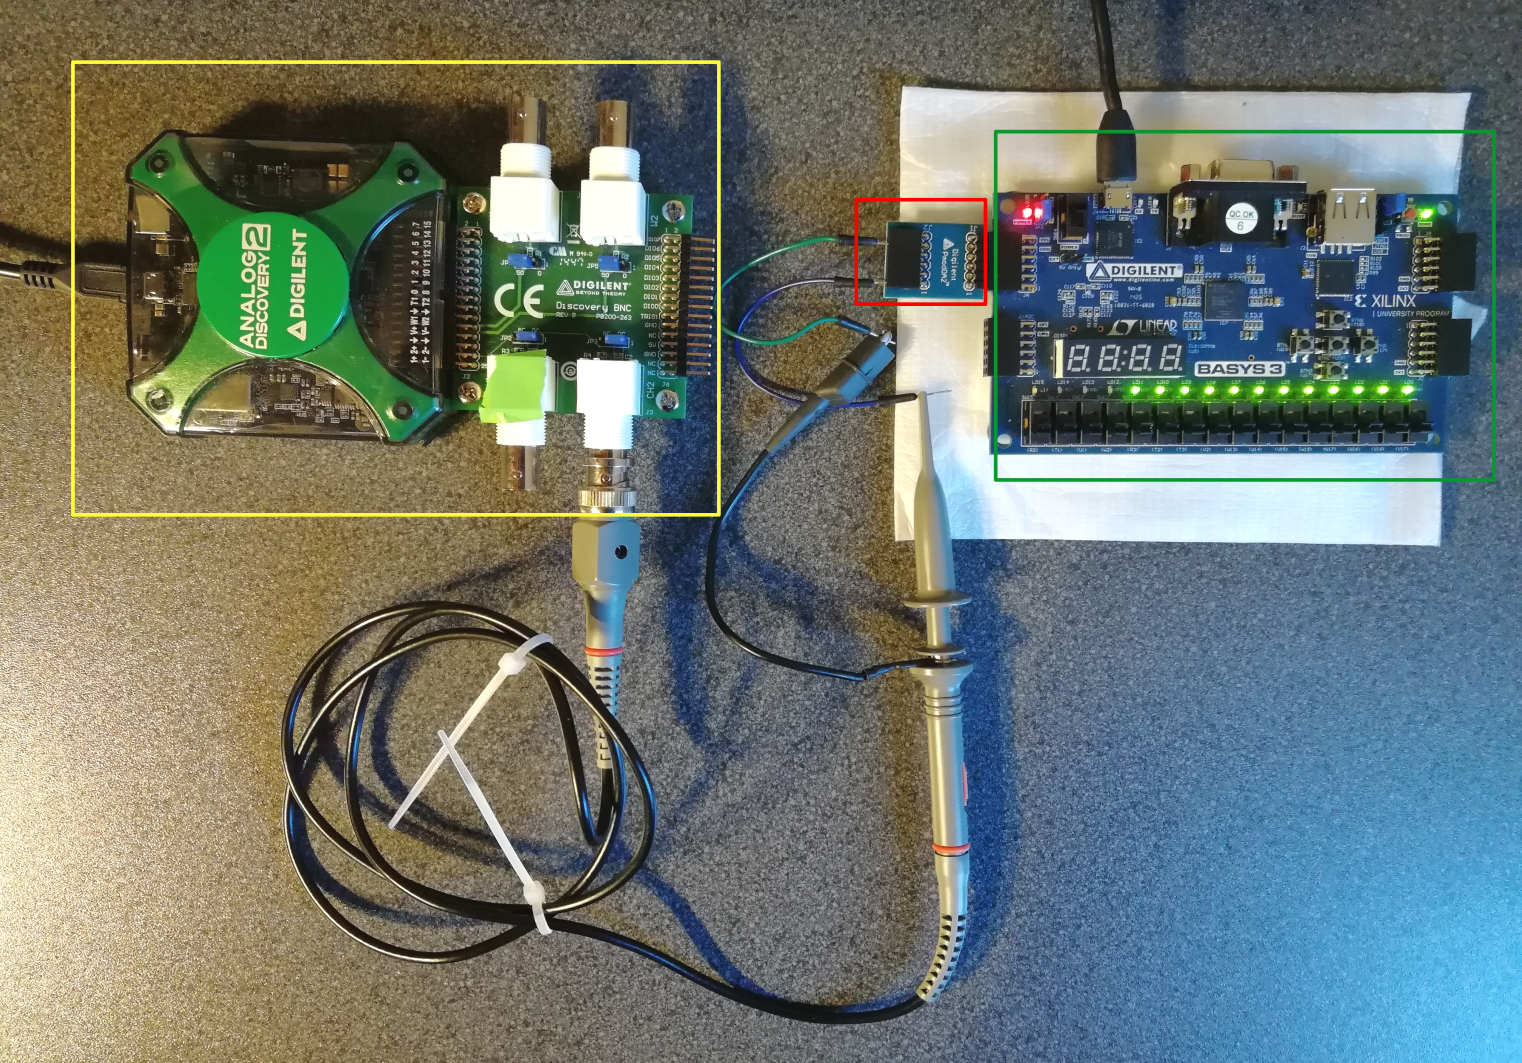
\includegraphics[scale=0.15]{testaufbau_annotated_fg}
  \end{figure}
\end{frame}

\begin{frame}{Funktionstest - Versuchsdurchführung}
  \begin{itemize}
  \item Ausführen und Kontrollieren von jedem Konfigurationsbefehl
  \item Jede Funktion einmal bei \SI{100}{\hertz} mit $U_{low} = \SI{0}{\volt}$ und $U_{high} = \SI{3.3}{\volt}$ messen
  \item Zick-Zack-Funktion zur Kontrolle des Frequenzbereichs mit folgenden Frequenzen $f$:
    \begin{table}
      \resizebox{0.95\textwidth}{!}{
        \begin{tabular}{|l|r|r|r|r|r|r|r|r|r|r|}
          \hline
          $f$ in Hz & 0,08 & 0,1 & 1 & 10 & 100 & $10^3$ & $10^4$ & $10^5$ & $3,5 \cdot 10^5$ & $10^6$\\ \hline
        \end{tabular}
      }
    \end{table}
  \item $\SI{0.08}{\hertz} < f_{min}$ und $\SI{1}{\mega\hertz} > f_{max}$
  \end{itemize}

\end{frame}

\pgfplotsset{
  no markers,
  scaled x ticks=false,
  grid=major,
  x unit=\second,
  y unit=\volt,
  ymin=-0.2, ymax=3.5,
  ytick={0, 0.55, 1.10, 1.65, 2.20, 2.75, 3.30},
  yticklabels={0, , 1.10, , 2.20, , 3.30},
}

\begin{frame}{Funktionstest - Funktionsverläufe bei \SI{100}{\hertz}}
  \begin{itemize}
    \item Frequenz wird korrekt ausgegeben
    \item \SI{0}{\volt} wird unterschritten und \SI{3.3}{\volt} nicht erreicht
  \end{itemize}
  \begin{figure}[h]
      \begin{tikzpicture}
        \pgfplotsset{
          xmin=-0.0075, xmax=0.0075,
          xtick={-0.0075, -0.005, -0.0025, 0, 0.0025, 0.005, 0.0075},
          xticklabels={-7.5, -5, -2.5, 0, 2.5, 5, 7.5},
          width=0.5\textwidth,
          height=4cm,
          x unit prefix=\milli}

        \begin{groupplot}[group style={
            group size=2 by 2,
            x descriptions at=edge bottom,
            xlabels at=edge bottom,
            y descriptions at=edge left,
            horizontal sep=1cm,
            vertical sep=0.5cm}]

          % const
          \nextgroupplot[use units=false]
          \addplot table [x=Time (s), y=Channel 2 (V), col sep=comma, row sep=newline] {../test/const100Hz_small.csv};
          % square
          \nextgroupplot 
          \addplot table [x=Time (s), y=Channel 2 (V), col sep=comma, row sep=newline] {../test/square100Hz_small.csv};
          % zigzag
          \nextgroupplot[
          xlabel=Zeit $t$,
          every axis x label/.append style={at=(ticklabel cs:1.1)},
          ylabel=Spannung $U(t)$,
          every axis y label/.append style={at=(ticklabel cs:1.1)}] 
          \addplot table [x=Time (s), y=Channel 2 (V), col sep=comma, row sep=newline] {../test/zigzag100Hz_small.csv};
          % ramp
          \nextgroupplot[use units=false]
          \addplot table [x=Time (s), y=Channel 2 (V), col sep=comma, row sep=newline] {../test/ramp100Hz_small.csv};
        \end{groupplot}
      \end{tikzpicture}
  \end{figure}
\end{frame}

\begin{frame}{Funktionstest - Kontrolle des Frequenzbereichs}

  \begin{itemize}
    \item bei $f < f_{min}$ kommt es zu Aliasing
    \item bei $f > f_{max}$ wird konstant \SI{0}{\volt} ausgegeben
    \item bei $f > \SI{10}{\kilo\hertz}$: starke Abweichung von idealer Kurve ab
    \begin{itemize}
      \item reduzierte Auflösung, Trägheit des DACs
    \end{itemize}  
  \end{itemize}
  \begin{figure}
    \pgfplotsset{xmin=-0.0000075,
                 xmax=0.00001,
                 xtick={-0.0000075, -0.000005, -0.0000025, 0, 0.0000025, 0.000005, 0.0000075, 0.000010},
                 xticklabels={, -5, , 0, , 5, , 10},
                 x unit prefix=\micro,
                 width=0.95\textwidth,
                 height=3.5cm}

    \begin{tikzpicture}
      \begin{groupplot}[group style={
          group size=1 by 2,
          x descriptions at=edge bottom,
          y descriptions at=edge left,
          horizontal sep=1cm,
          vertical sep=0.8cm}]
        \nextgroupplot[use units=false, title=\SI{100}{\kilo\hertz}]
        \addplot[color=blue] table[x=Time (s), y=Channel 2 (V), col sep=comma, row sep=newline] {../test/zigzag100000Hz_5cyc.csv};
        \addplot[color=red] table [x=x, y=y, col sep=comma, row sep=newline] {idealzigzag100.csv};

        \nextgroupplot[title=\SI{350}{\kilo\hertz},
                       xlabel=\small Zeit $t$,
                       ylabel=\small Spannung $U(t)$,
                       every axis y label/.append style={at=(ticklabel cs:1.2)}] 
        \addplot[color=blue] table [x=Time (s), y=Channel 2 (V), col sep=comma, row sep=newline] {../test/zigzag350000Hz_5cyc.csv};
        \addplot[color=red] table [x=x, y=y, col sep=comma, row sep=newline] {idealzigzag350.csv};
        \end{groupplot}
      \end{tikzpicture}
    \end{figure}
    
\end{frame}

\section{Fazit}
\begin{frame}{Fazit}
  \begin{itemize}
  \item UART-Schnittstelle funktioniert
  \item Generierung von Funktionen
    \begin{itemize}
      \item zuverlässig von \SI{0.1}{\hertz} bis \SI{10}{\kilo\hertz}
      \item darüber hinaus sehr unsaubere Funktionsverläufe
        \begin{itemize}
        \item sinkende Auflösung
        \item evtl. zu langsame Änderung des DAC-Ausgangswerts
        \end{itemize}
      \item $U_{high}$ und $U_{low}$ scheinen verschoben zu sein
      \begin{itemize}
        \item evtl. ungenaue Referenzspannung, da Referenzspannung der Versorgungsspannung entspricht
      \end{itemize}
      \end{itemize}
  \end{itemize}
\end{frame}

\begin{frame}{Referenzen}
  Source Code, Anleitung und Python Interface:\\ 
  \href{https://github.com/markushart/studienarbeit_function_generator.git}{\small\texttt{https://github.com/markushart/studienarbeit\_function\_generator.git}}
\end{frame}

\begin{frame}{Komponenten - Rechteck}
  \begin{itemize}
  \item nach 68 steigenden Flanken \emph{Counter} aktivieren
  \item Ausgang auf \emph{low} wenn \emph{o\_count} $>$ \emph{thresh}, sonst \emph{high} 
  \end{itemize}
  \begin{figure}
    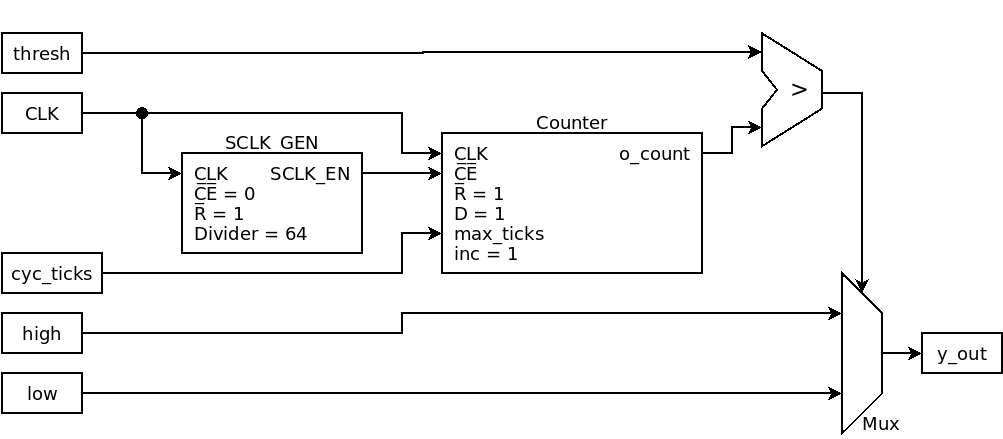
\includegraphics[scale=0.32]{square}
  \end{figure}
\end{frame}

\begin{frame}{Komponenten - Digital-Analog-Konverter}
  \begin{itemize}
  \item Implementierung des PmodDA2-Protokolls
    \begin{itemize}
    \item $\overline{\mbox{SYNC}}$: Chip-Enable Signal für den DAC
    \item DINA, DINB: serielle DAC-Daten, aktuell nur Kanal A genutzt
    \item CLK: DAC-Clock läuft mit \SI{25}{\mega\hertz}
    \end{itemize}
  \end{itemize}
  \begin{figure}[h] \centering
    \begin{tikztimingtable}
      Bit Nr.                   & 17{2D{\hexcountmakro}} [white] \\ 
      parallele Daten           & 33D{0x123}D{}                  \\
      CLK                       & 34{C}                          \\
      $\overline{\mbox{SYNC}}$  & H 32L H                        \\
      DINA                      & 5X 4L 6L 2H 4L 2H 2L 4L 4H L   \\
      \extracode
      \vertlines[help lines]{0, 2, ..., 34}

    \end{tikztimingtable}
  \end{figure}
\end{frame}

\begin{frame}{Zick-Zack bei $f < f_{min}$ und $f > f_{max}$}
  \begin{itemize}
  \item Frequenzbereich:
    \begin{itemize}
    \item $f_{min} = \SI{0.0877}{\hertz}$
    \item $f_{max} = \SI{367.5}{\kilo\hertz}$ für die Zick-Zack Funktion
    \item $f_{max} = \SI{735}{\kilo\hertz}$ für Rampe und Rechteck
    \end{itemize}
  \item bei $f < f_{min}$ ist Ausgangsfrequenz \SI{20.5}{\hertz}
    \begin{itemize}
    \item interner Zählstand für \emph{cyc\_ticks} nicht mehr darstellbar
    \end{itemize}
  \item bei $f > f_{max}$ wird konstant \SI{0}{\volt} ausgegeben
    \begin{itemize}
    \item $\emph{cyc\_ticks} / 2 = 1$, \emph{direction} wird nicht mehr getoggelt
    \end{itemize}
  \end{itemize}
\end{frame}

\end{document}